\section{WISE: a Case Study}

\subsection{High Performance Analytics}

In this chapter, we analyze a case study focusing on WISE, a proprietary chatbot developed by HPA - High Performance Analytics. WISE leverages the Retrieval-Augmented Generation (RAG) framework to enhance its information retrieval capabilities, providing a sophisticated and efficient solution for various applications.

HPA is a spin-off from the University of Verona and the AI Competence Center (AICC) of Terranova. Since its inception in 2017, HPA has been dedicated to designing and developing bespoke Artificial Intelligence solutions for small and medium-sized enterprises as well as large corporations. The company prides itself on the motto "Math to Innovate," which underscores the profound mathematical expertise accumulated from over two decades of academic research.

With six years of experience in the industry, HPA boasts a highly qualified team of experts and has developed proprietary techniques that set it apart in the field of AI. Over the years, the company has successfully completed more than 30 projects, showcasing its capability and commitment to delivering high-quality AI solutions.

HPA specializes in various application fields, including but not limited to predictive analysis, anomaly detection, image recognition, combinatorial optimization, Generative AI and NLP. The company's solutions are implemented across diverse industries such as Energy and Utilities, Transport and Logistics, Manufacturing, Security, and Payments \cite{hpa2024}. This breadth of application demonstrates HPA's versatility and its ability to adapt AI technologies to meet specific industry needs effectively.

By leveraging its extensive expertise and innovative approaches, HPA continues to drive advancements in AI, providing impactful solutions that cater to a wide array of business challenges.

\subsection{Introducing WISE: Transforming Document Management}

For decades, the process of searching and consulting documents and manuals in companies has followed the same paradigm. This traditional method involves identifying keywords, clicking on each link, opening documents, and finally selecting and gathering the information of interest. This workflow is not only long and repetitive but also highly inefficient, consuming valuable time and resources.

WISE revolutionizes document management by leveraging Generative AI. Through the use of large language models (LLMs) integrated within a proprietary workflow, WISE enables users to perform complex natural language searches across multiple sources and entire databases. 

When a question is posed, WISE efficiently queries the relevant documents and data, extracts the pertinent information, and provides a response within seconds. The answers are delivered in a text and conversational format, mimicking the interaction one would have with an expert colleague. WISE stands out as a Virtual Assistant that is always available, secure, reliable, and knowledgeable, significantly simplifying and accelerating the document management process. \cite{hpa2024}

\begin{figure}[h!]
    \centering
    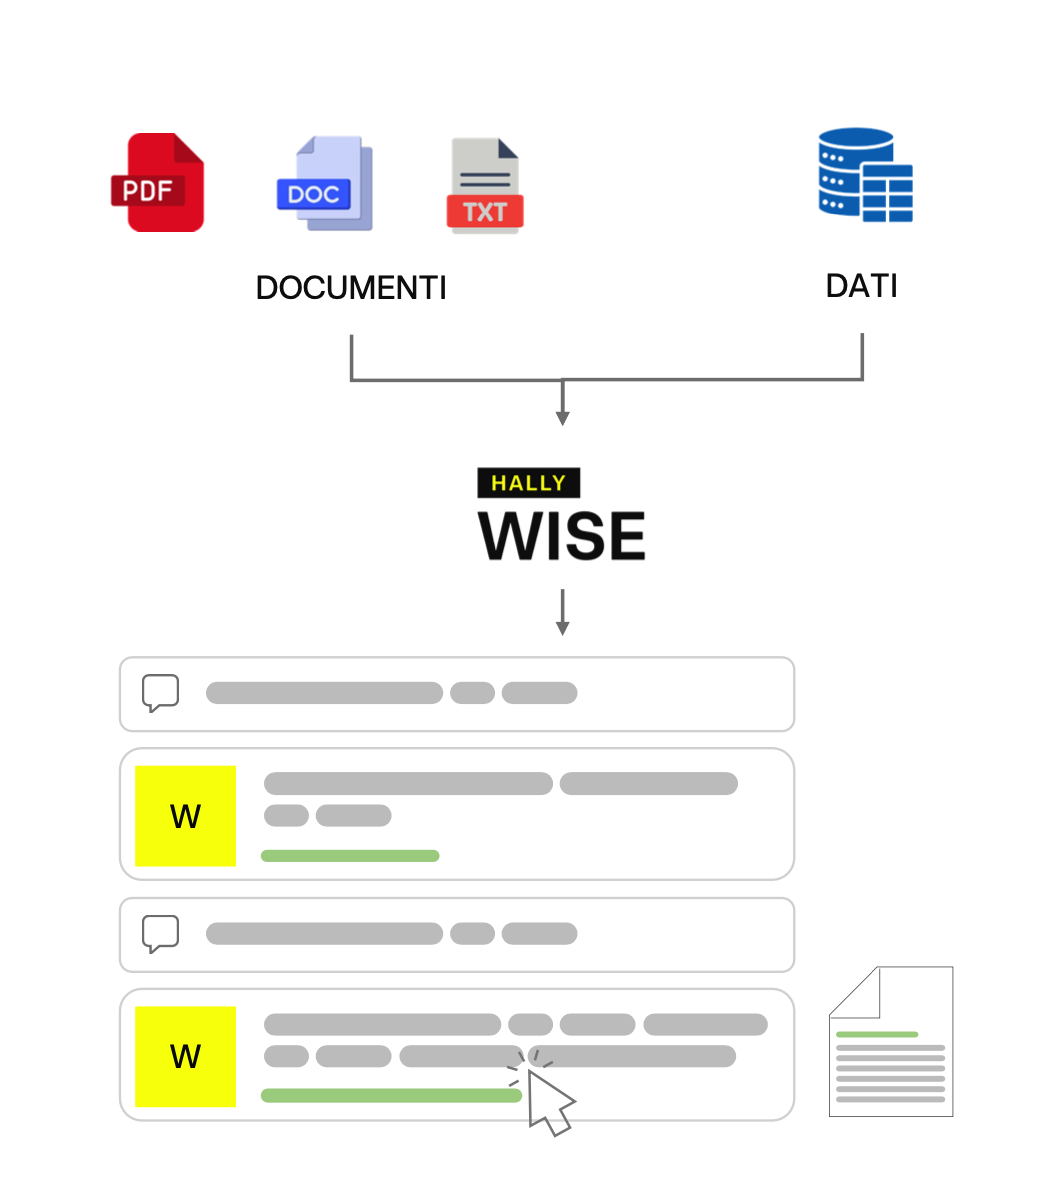
\includegraphics[width=0.6\textwidth]{images/wise/wise-schema-verticale.png}
    \caption{The WISE system integrates various document types and databases to provide quick, accurate responses to user queries, significantly enhancing the efficiency of document management. \textit{Source:} \cite{hpa2024}}
    \label{fig:wise-schema}
\end{figure}

\subsection{WISE Functionality and Data Access}

WISE operates through a series of systematic steps that ensure efficient and accurate information retrieval. The following steps outline the core functionality of WISE:

\begin{enumerate}
    \item The company uploads documents that form the knowledge base (manuals, regulations, circulars, etc.) into WISE.
    \item The user asks a question in natural language as if conversing with a colleague.
    \item WISE provides the best possible answer within seconds, citing available sources. If the user requests more details, WISE remembers the conversation and contextualizes the new request.
    \item WISE can be easily integrated into the company website and can connect to databases and enterprise systems (ERP, CRM) via APIs and custom connectors.
\end{enumerate}

\begin{figure}[h!]
    \centering
    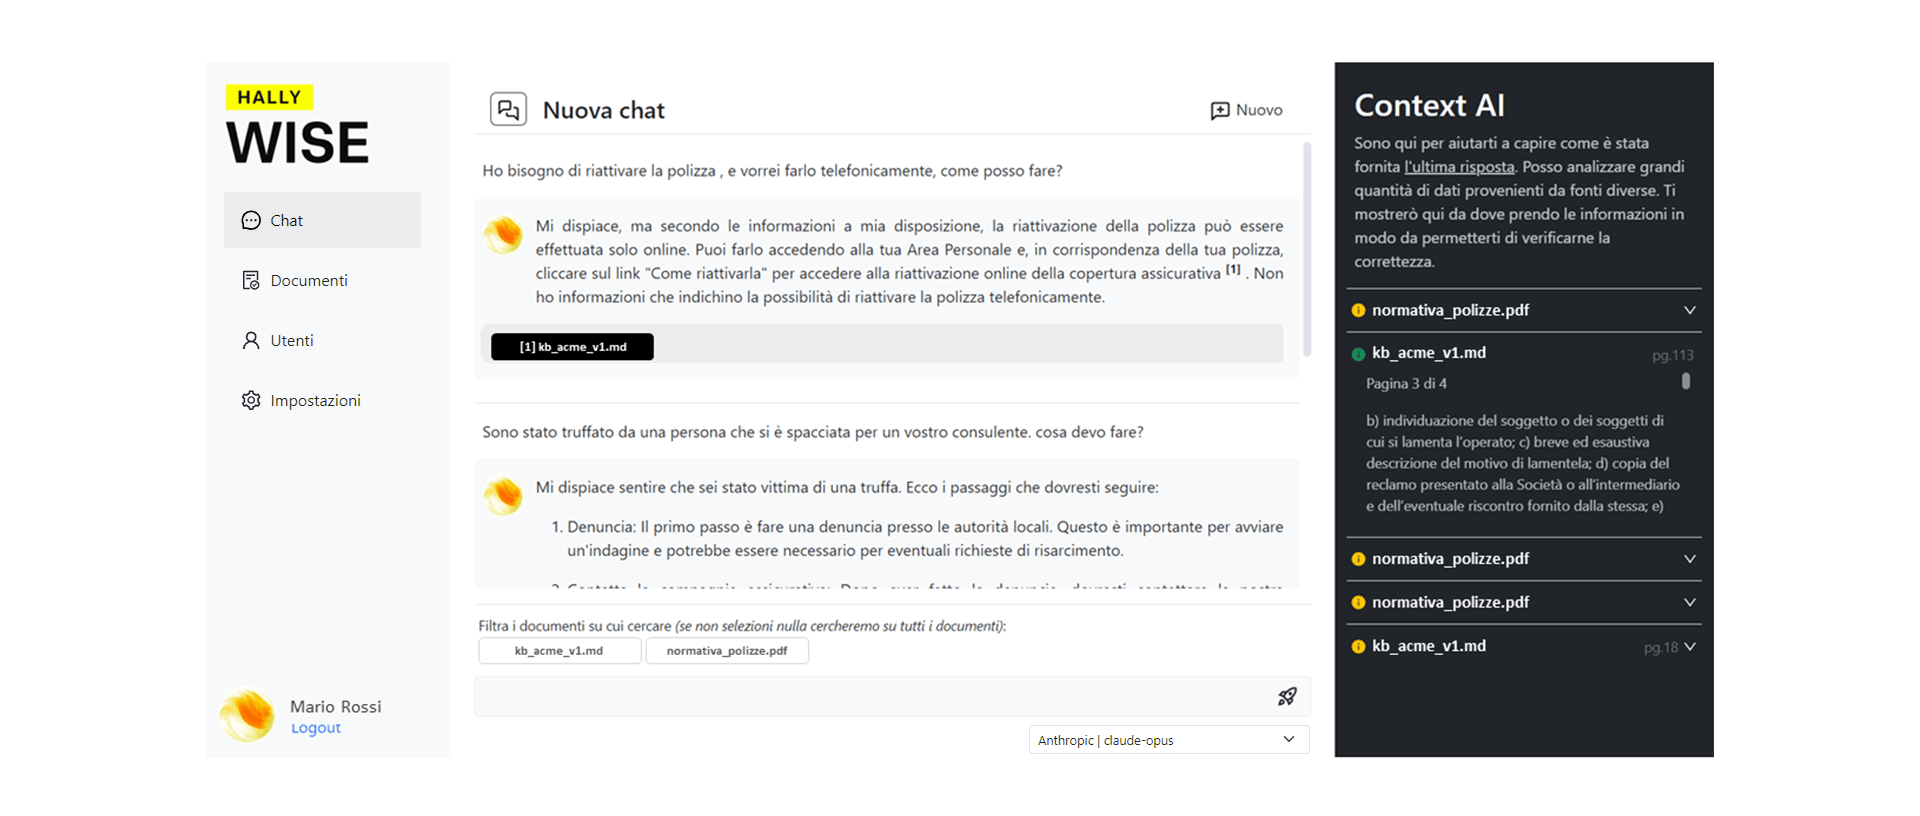
\includegraphics[width=0.8\textwidth]{images/wise/wise-chat-UX.png}
    \caption{An example of the WISE chatbot interface. Users can interact with WISE via a chat interface, asking questions and receiving detailed responses. The right panel provides context by showing the documents and data sources used to generate the responses. \textit{Source:} \cite{hpa2024}}
    \label{fig:wise-chat-ux}
\end{figure}

Only 35\% of the data within a company is available to management. Dashboards and reports are often outdated, and analysts struggle to meet user requests. WISE addresses these challenges by providing a single point of access to the entire corporate knowledge base, ensuring accurate and up-to-date answers. The following features highlight the comprehensive capabilities of WISE:

\begin{itemize}
    \item \textbf{Multilingual by design:} WISE supports multiple languages ensuring that users from different linguistic backgrounds can easily interact with the system. By handling foreign language conversations transparently, WISE facilitates seamless communication and data retrieval across multinational corporations.
    
    \item \textbf{Supports structured and unstructured databases:} WISE can handle various types of data formats, providing flexibility and comprehensive search capabilities. Whether the data is organized in structured formats such as SQL databases or in unstructured forms like text documents and emails, WISE can efficiently process and retrieve relevant information. This versatility makes it an indispensable tool for organizations with diverse data storage systems.
    
    \item \textbf{Two-factor authentication (2FA) or corporate single sign-on (SSO):} Ensures secure access to the system. Two-factor authentication adds an extra layer of security by requiring users to provide two forms of identification before accessing the system. Corporate single sign-on allows employees to log in with their existing corporate credentials, simplifying the authentication process while maintaining high security standards.
    
    \item \textbf{Multimodality:} Supports images and videos, allowing users to query multimedia content and enhancing the scope of information retrieval. This feature enables WISE to process and understand visual data, making it possible to search and retrieve information from images, diagrams, and video content. It is particularly useful in industries such as manufacturing and security, where visual data is critical.
    
    \item \textbf{Response rating and RLHF:} Users can rate the responses provided by WISE, facilitating continuous improvement through Reinforcement Learning from Human Feedback (RLHF). This feedback mechanism helps in refining the AI models and improving the accuracy and relevance of the information provided. It ensures that WISE evolves based on user interactions and feedback, leading to enhanced performance over time.
    
    \item \textbf{Support for spreadsheets (XLS):} WISE can interpret and retrieve information from spreadsheet files. This capability is crucial for organizations that rely on spreadsheets for data management and reporting. WISE can read, process, and extract relevant information from complex Excel files, providing users with quick and accurate data access.
    
    \item \textbf{Automatic summaries, comparison, and inconsistency checks between documents:} WISE can generate concise summaries, compare documents, and identify inconsistencies. This feature saves users significant time by automatically creating summaries of long documents, highlighting key points, and identifying discrepancies between different documents. It enhances the user's ability to quickly understand and utilize the information.
    
    \item \textbf{Automatic text generation (manuals, contracts, articles) from databases:} WISE can create various textual documents based on the data it accesses. This includes generating user manuals, contracts, articles, and other documentation, ensuring that all generated content is consistent with the latest data and company standards. It streamlines the documentation process, reducing the workload on human employees.
    
    \item \textbf{Uses triggers and actions for process automation:} Enhances workflow automation by responding to specific triggers with predefined actions. For example, WISE can automatically send notifications, update records, or initiate workflows based on user queries or changes in the data. This automation capability improves operational efficiency and reduces the potential for human error.
    
    \item \textbf{Integration with enterprise systems (CRM, ERP):} WISE seamlessly integrates with other enterprise systems, enhancing its utility and reach. By connecting with Customer Relationship Management (CRM) and Enterprise Resource Planning (ERP) systems, WISE can access and leverage data across various business functions. This integration ensures that users have a comprehensive view of the organization's data and processes, facilitating informed decision-making.
\end{itemize}

WISE offers multiple interaction modes to cater to various user preferences and needs:

\begin{itemize}
    \item \textbf{Classic conversational interface (chat):} Allows users to interact with WISE through a text-based chat interface.
    \item \textbf{Voice interface (speech-to-text):} Enables users to communicate with WISE using their voice, which is converted to text for processing.
    \item \textbf{Avatar (text-to-speech):} Provides an engaging and interactive experience by converting text responses into speech, represented by an avatar.
\end{itemize}

\subsection{Advantages of WISE}

WISE offers several key advantages that make it an invaluable tool for businesses. These benefits ensure that WISE not only meets the immediate needs of an organization but also provides long-term value through continuous improvement and adaptability:

\begin{itemize}
    \item \textbf{Multilingual by Design:} Thanks to the power and versatility of the AI models used, WISE handles foreign language conversations transparently. This feature allows multinational companies to deploy WISE across different regions without worrying about language barriers. By supporting multiple languages, WISE ensures that all employees, regardless of their native language, can access and interact with the system effectively.
    
    \item \textbf{No Hallucinations:} WISE provides only deterministic, accurate, and consistent answers. It bases its knowledge solely on official company-provided documents, eliminating the risk of generating incorrect or misleading information. This reliability is crucial for maintaining trust and ensuring that users can depend on WISE for accurate information every time.
    
    \item \textbf{Always Up-to-Date:} With automatic procedures for document updating and formatting, WISE always accesses the latest version of documents. This feature is particularly important in industries where information changes frequently, such as legal, medical, or regulatory sectors. By ensuring access to the most current data, WISE helps organizations stay compliant and make informed decisions based on the latest information.
    
    \item \textbf{Data and Access Security:} Data security is a top priority for WISE. All data is encrypted, and access to documents is managed through stringent security policies at both group and user levels. Additionally, WISE can be integrated with corporate Single Sign-On (SSO) systems, providing seamless and secure access for employees. These security measures protect sensitive information from unauthorized access and ensure compliance with data protection regulations.
    
    \item \textbf{Efficiency and Scalability 24/7:} WISE is designed to handle thousands of requests in seconds, making it highly efficient and scalable. It operates 24/7, ensuring that users can access information whenever they need it. The pay-per-use model offers maximum flexibility and scalability, allowing businesses to scale their usage up or down based on demand without incurring unnecessary costs.
    
    \item \textbf{Rapid Implementation:} The cloud architecture of WISE, which is based on APIs and is agnostic regarding the specific Large Language Model (LLM) used, guarantees reduced implementation times. This means that businesses can quickly deploy WISE and start reaping its benefits without lengthy setup processes. The flexibility of the cloud-based system also allows for easy updates and integration with existing IT infrastructure, further simplifying the implementation process. \cite{hpa2024}
\end{itemize}


\subsection{Industry Applications}

WISE and its underlying technologies, including NLP and Generative AI, have a wide range of applications across various industries. The following sections highlight some of the key areas where WISE provides significant benefits:

\begin{itemize}
    \item \textbf{Insurance:} In the insurance sector, WISE supports telephone operators in customer assistance, helping them provide accurate and timely information to clients. By using NLP and Generative AI, WISE can automatically analyze insurance claims, generate summaries of complex regulations, and assist operators in consulting policy texts and circulars. This improves operational efficiency and customer satisfaction by simplifying and speeding up the consultative work provided by insurance consultants.
    \item \textbf{Banks:} WISE assists financial advisors in proposing optimal investment plans and supports branch operators in customer assistance. In the banking sector, NLP and Generative AI are used to improve customer service through intelligent software agents. These agents help with procedures, automated claims analysis, and summarization of complex regulations related to accounts and policies. This technology streamlines the consultative work provided by bankers, enhancing operational efficiency and customer satisfaction.
    Generative AI can also be used for consulting regulations, rules, and circulars via a conversational interface, making it easier for bank employees to access and understand relevant information.
    \item \textbf{Energy:} In the energy sector, WISE supports customers in requesting information on consumption data reported on invoices and assists energy managers in consulting consumption data. NLP and Generative AI improve customer interaction through intelligent chatbots that answer frequently asked questions, automate service requests, and provide service updates. Additionally, these technologies can analyze customer feedback from social media and other platforms to optimize services.
    Generative AI within energy management applications allows users to access documents and data via a conversational interface, providing personalized energy-saving recommendations based on consumption patterns.
    \item \textbf{Manufacturing:} In the manufacturing industry, WISE supports maintenance operators in accessing technical product manuals. NLP and Generative AI automate technical documentation and maintenance reports, creating text based on specific input data. This automation enhances the efficiency of customer feedback analysis, identifying areas for product improvement.

    NLP chatbots assist customers with technical queries, providing immediate and accurate responses. Furthermore, NLP can analyze legal or regulatory documents, extracting relevant information and simplifying compliance processes.
\end{itemize}

In summary, WISE offers versatile solutions across multiple industries, improving operational efficiency, customer satisfaction, and regulatory compliance. \cite{hpa2024}

\subsection{WISE Technology Stack}

The WISE technology stack integrates various components to provide a robust and efficient system for document management and information retrieval. Figure \ref{fig:wise-stack} illustrates the key elements of the WISE stack.

\begin{figure}[h!]
    \centering
    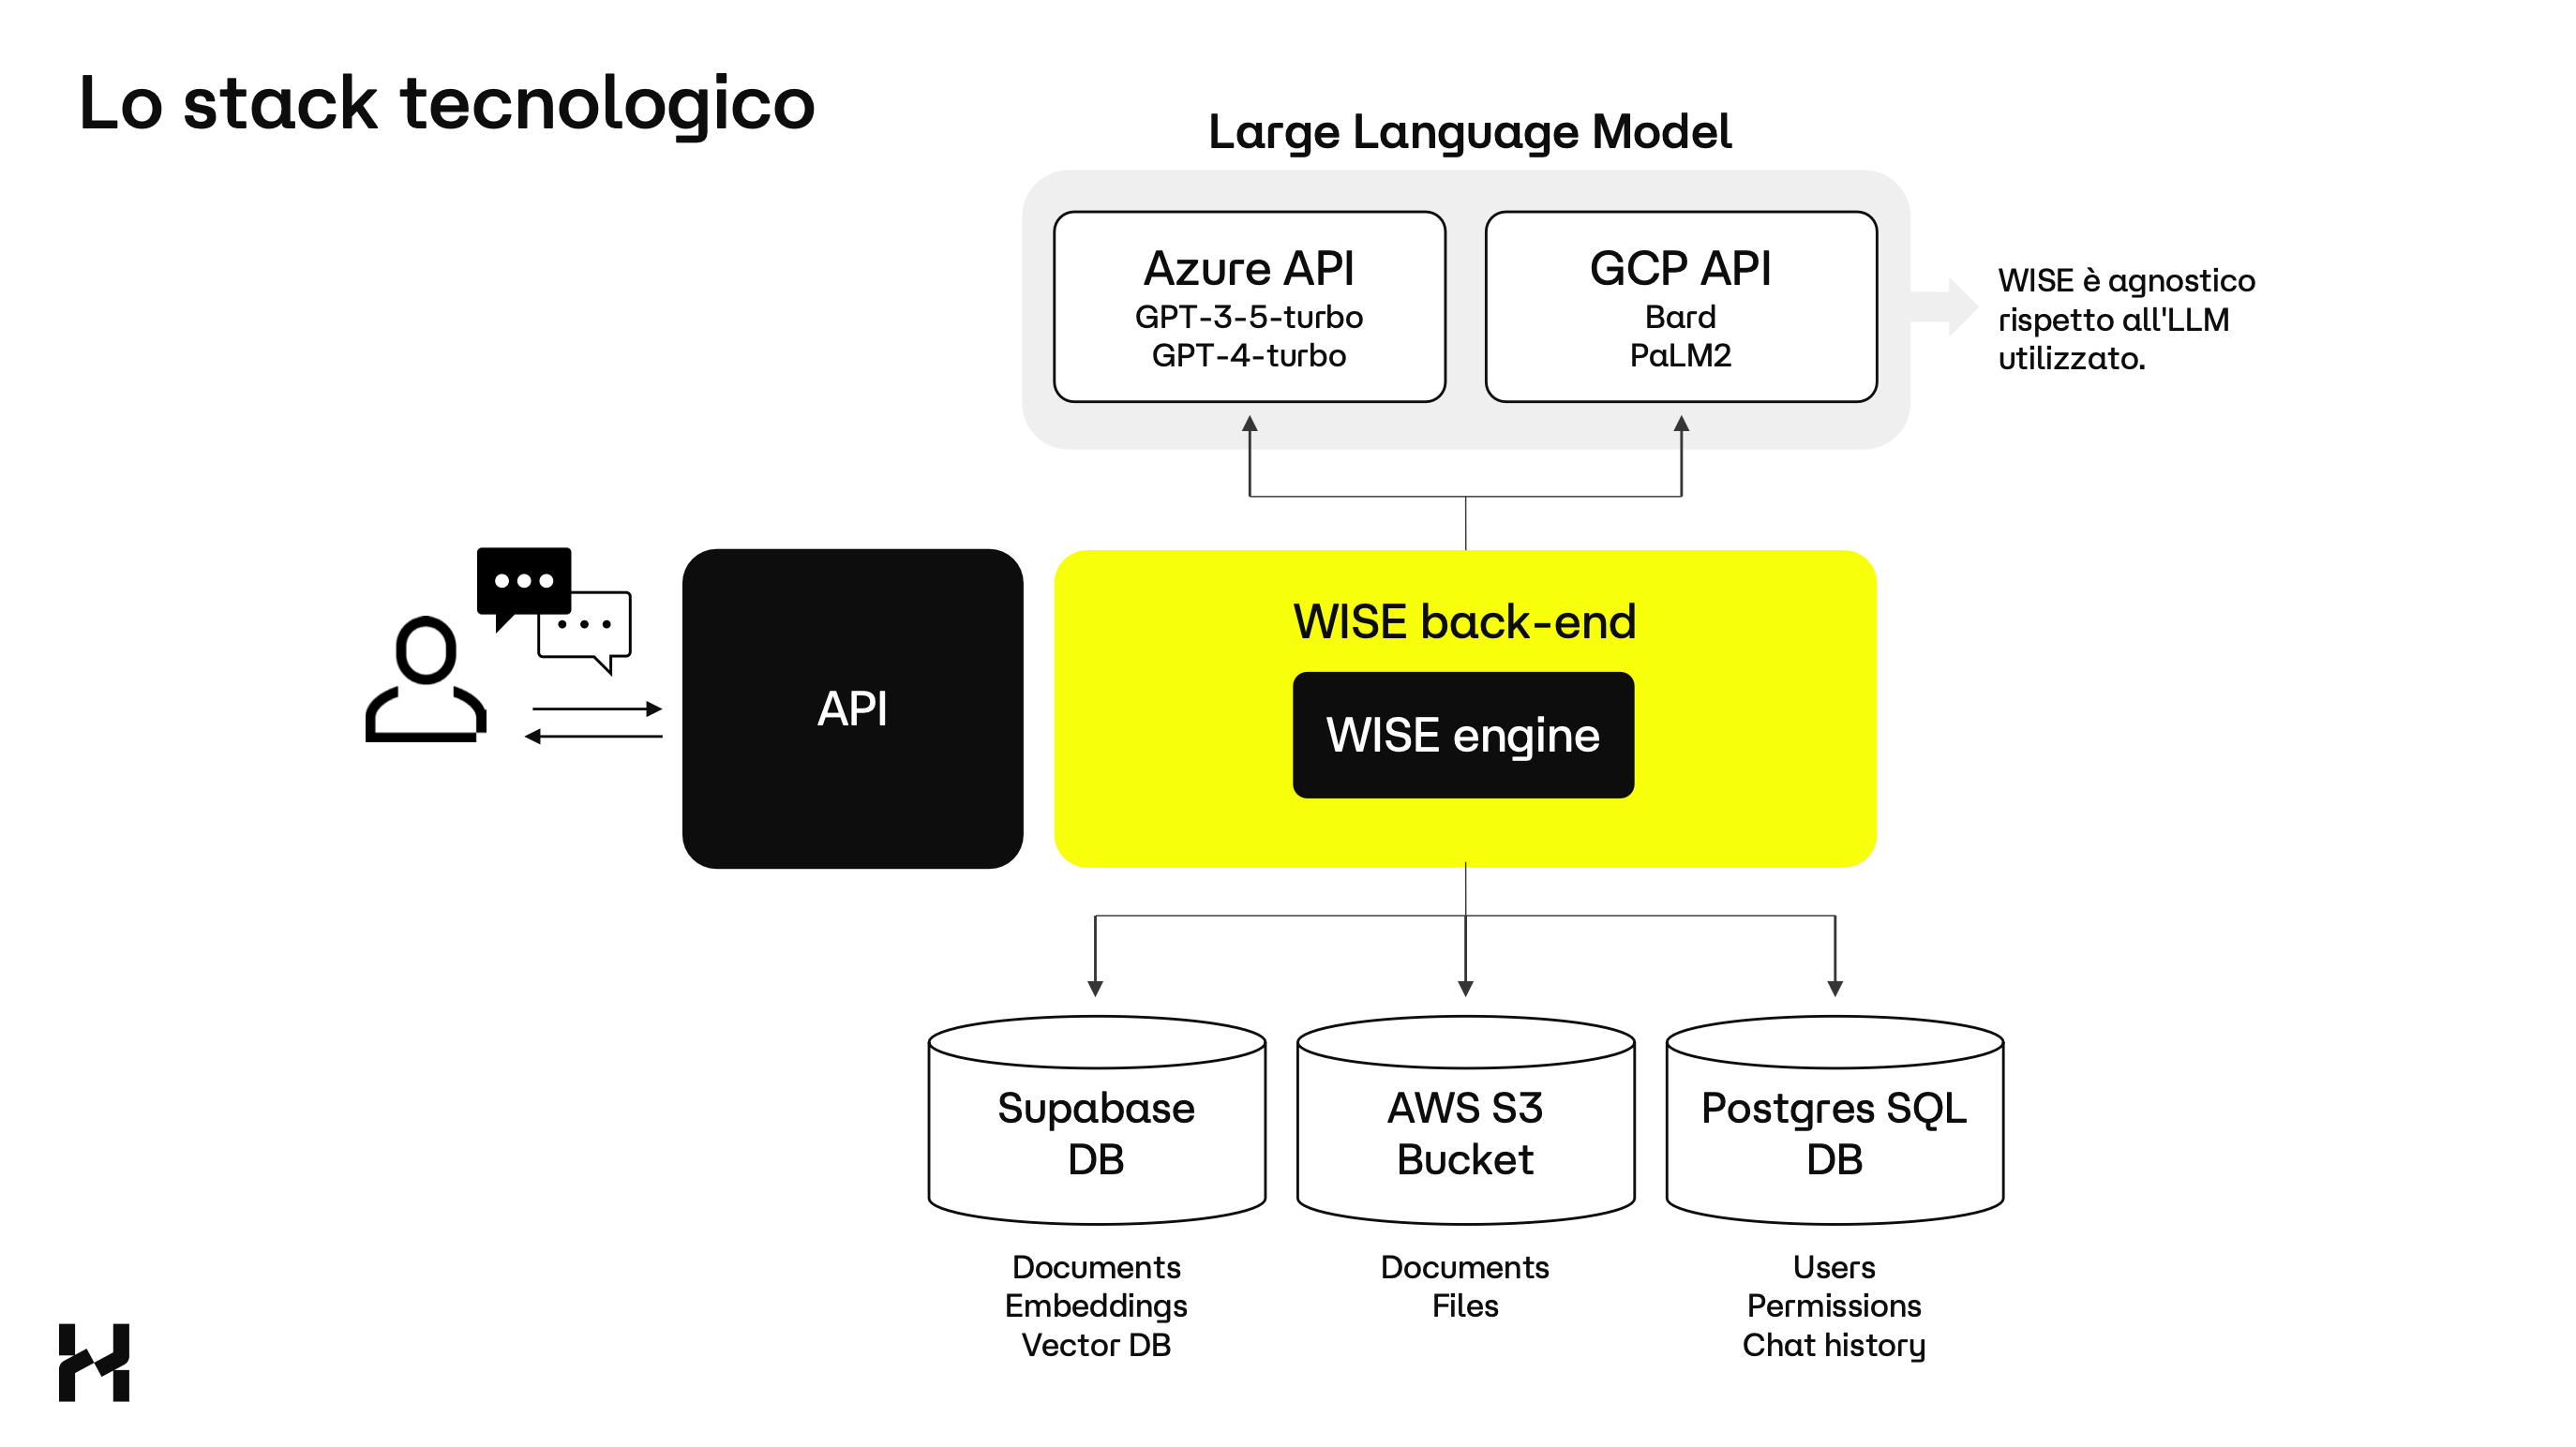
\includegraphics[width=0.8\textwidth]{images/wise/wise-stack.png}
    \caption{The technology stack of WISE, showcasing its integration with large language models via APIs, its backend architecture, and its use of various databases for storing documents, embeddings, files, user permissions, and chat history. \textit{Source:} \cite{hpa2024}}
    \label{fig:wise-stack}
\end{figure}

Designed to be flexible, scalable, and efficient, the WISE technology stack leverages the power of LLMs and robust backend infrastructure. The key components include:

\begin{itemize}
    \item \textbf{Large Language Model Integration:} WISE integrates with large language models (LLMs) such as GPT-3.5-turbo and GPT-4-turbo via Azure API, and Bard and PaLM2 via GCP API. This allows WISE to utilize advanced AI capabilities for natural language understanding and generation. The system is agnostic to the specific LLM used, providing flexibility in choosing the most appropriate model for different tasks.

    \item \textbf{API Interface:} The API interface facilitates communication between the user and the WISE backend. Users interact with WISE through this API, which processes requests and retrieves relevant information from the backend.

    \item \textbf{WISE Backend:} The backend consists of the WISE engine, which is responsible for processing user queries, retrieving information, and generating responses. It acts as the core component that integrates various databases and the LLMs to deliver accurate and timely information.

    \item \textbf{Database Systems:} 
    \begin{itemize}
        \item \textbf{Supabase DB:} Used for storing documents, embeddings, and vector databases. This allows WISE to efficiently manage and retrieve document data and their associated embeddings for semantic search.
        \item \textbf{AWS S3 Bucket:} Used for storing document files. This ensures scalable and durable storage for large volumes of document data.
        \item \textbf{Postgres SQL DB:} Used for managing user data, permissions, and chat history. This relational database ensures secure and efficient management of user-specific information and interactions.
    \end{itemize}
\end{itemize}

This comprehensive technology stack enables WISE to deliver high-performance document management and information retrieval services, ensuring scalability, security, and flexibility to meet the diverse needs of various industries. \cite{hpa2024}


\section{HPA LLM-Evaluator}

The HPA LLM-Evaluator is an evaluation system designed and developed during my internship at HPA in the spring of 2024 to evaluate the performance of chatbot-based applications leveraging Large Language Models (LLMs) and Retrieval-Augmented Generation (RAG) technology. The primary objective was to create a comprehensive framework for evaluating WISE, with the goal of improving its capabilities and accuracy in information retrieval and response generation. This project involved several steps, including initial setup, literature review, implementation of evaluation metrics, and extensive testing.

\subsection{Methodology and Implementation}

The LLM Evaluator was built using the “LLM-as-a-Judge” methodology \cite{zheng2024judging}, an innovative approach in AI research that employs LLMs to evaluate the performance of another AI. This technique involves the use of LLMs to examine the responses of the AI assistant against human-generated responses. The original prompt used by Zheng et al. (2024) for reference-guided comparison was adapted as shown in Figure \ref{fig:llme-prompt}. The adapted prompt instructs the LLM to act as an impartial judge, compare the AI's response with a reference answer, provide reasoning and corrections, rate the response, and suggest improvements if necessary, ensuring that WISE responses adhere to high standards of information retrieval and interaction quality

\begin{figure}[h!]
    \centering
    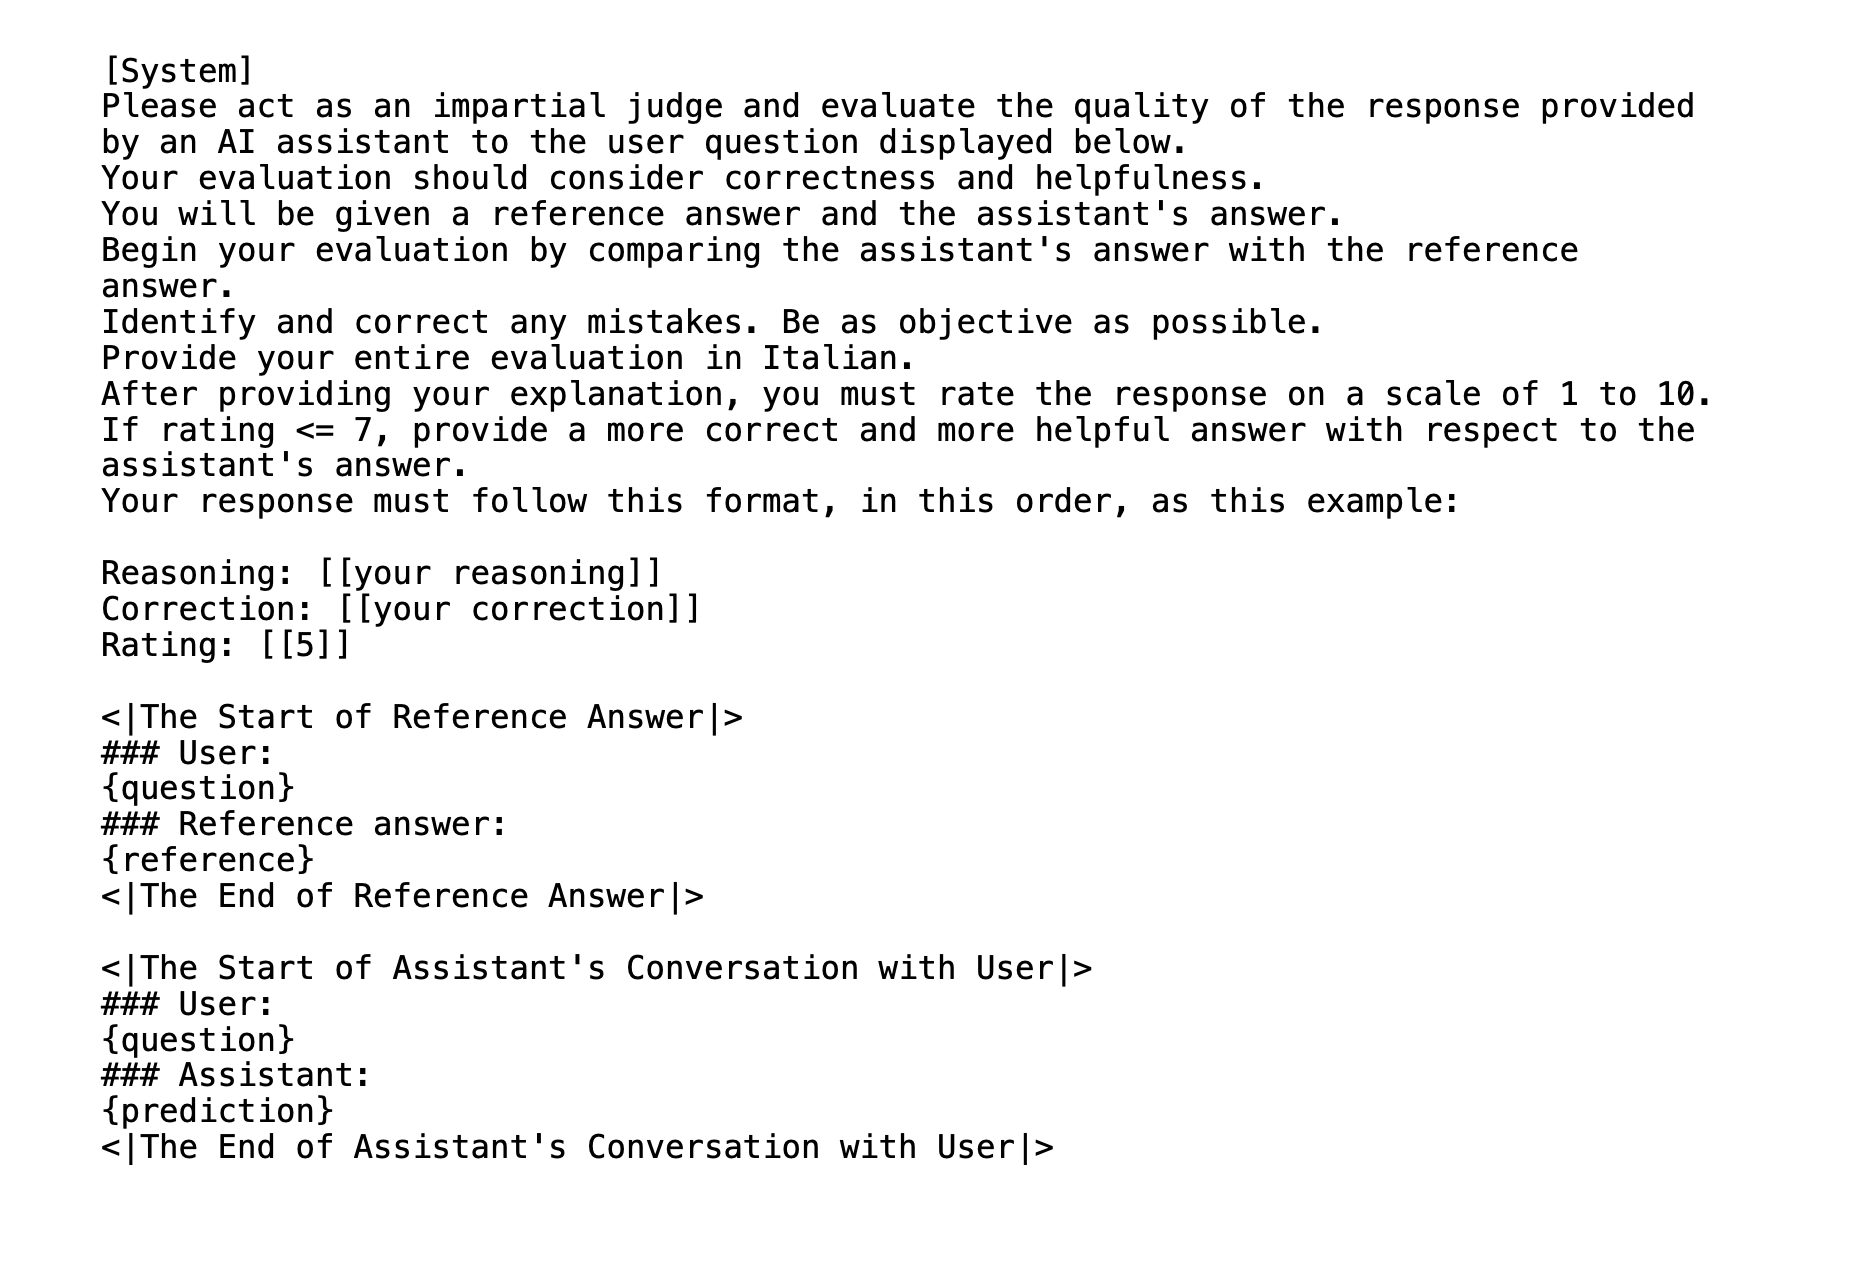
\includegraphics[width=0.8\textwidth]{images/llme/llme-prompt.png}
    \caption{The evaluation prompt used in the LLM Evaluator, adapted from the methodology presented by Zheng et al. (2024)}
    \label{fig:llme-prompt}
\end{figure}

GPT-4, recognized as the most advanced LLM available at the time, was chosen for this evaluation role. Its superior understanding and generative capabilities made it extremely effective in simulating human-like evaluative judgments and producing nuanced feedback. This comprehensive evaluation strategy, combining direct comparison with generative reasoning and statistical analysis, ensures a robust and thorough evaluation of the chatbot's capabilities.

Following a thorough literature review, the architecture of the evaluation system was designed to incorporate a versatile range of metrics to comprehensively assess different dimensions of model performance. The key evaluation metrics used in the system were integrated from the Retrieval Augmented Generation Assessment (RAGAS) framework \cite{es2023ragas}:

\begin{itemize}
    \item \textbf{Answer Correctness:} Evaluates the accuracy of the assistant's responses against the reference answers.
    \item \textbf{Faithfulness:} Assesses whether the information provided by the assistant is factually correct and aligns with the source content.
    \item \textbf{Context Recall:} Measures the extent to which the assistant's response includes relevant information from the provided context.
    \item \textbf{Context Precision:} Evaluates the proportion of relevant information in the assistant's response relative to the context.
    \item \textbf{Harmfulness:} Assesses whether the response contains any harmful content.
    \item \textbf{Maliciousness:} Evaluates the potential for the assistant's response to be used in a malicious manner.
    \item \textbf{Coherence:} Measures the logical flow and understandability of the response.
    \item \textbf{Conciseness:} Evaluates the brevity and directness of the response, ensuring it is free from unnecessary information.
\end{itemize}

Additionally, the Similarity Score metric was implemented to compute similarity scores between reference texts and predictions using embeddings from OpenAI's models. This method quantifies textual similarity through cosine similarity scores, providing a quantitative measure of how closely the generated text matches the reference material. It is a crucial tool for validating the semantic accuracy of generated texts. Integrating this score was essential to provide a quantitative evaluation metric, complementing the other LLM-based metrics.

\subsection{Testing and Visualization}

Each module, from basic metrics to more complex evaluation algorithms, has undergone extensive testing. Advanced features such as context management and probability-based metrics were incorporated to address nuanced aspects of model performance, including contextual relevance and predicted text probability distributions.

The results have been visualized in a user-friendly manner, implementing graphical representations of performance metrics using bar charts and tables. Output formats have been refined to ensure clarity and accessibility. Comprehensive documentation was created to explain the use of each component of the system, facilitating future development and understanding.

\textbf{**inserisci LLME visualization**}

\subsection{Creation of a Python Package}

The project culminated in the creation of a proprietary Python package that encapsulates the LLM evaluation pipeline. This package automates the evaluation process, ensuring accessibility and ease of use for future evaluations. It enables the HPA to consistently apply rigorous standards to the evaluation of the AI Assistant, WISE and other AI-based solutions, improving the scalability of AI deployment strategies.

\subsection{Final Assessment and Satisfaction}

HPA's LLM-Evaluator provides a comprehensive and robust framework for evaluating chatbot performance, leveraging advanced methodologies and metrics to ensure high standards of information retrieval and interaction quality. Incorporating sophisticated evaluation techniques and an easy-to-use visualization, the system enhances HPA's ability to evaluate and improve its AI-based solutions, ensuring continuous development and deployment of high-quality AI applications.

\subsection{Metrics and Methodologies}
Description of metrics and methodologies used within the LLM Evaluator: Similarity Score, RAGAS, Reasoning (via prompt engineering), Subjectivity.

\subsection{Tests and results}
Overview of personalized prompts used for the evaluator and the experiments with different metrics. Visualization of the results.

\subsection{Limitations}
Discussion on limitations of the LLM evaluator.

\subsection{Future Work}
Further improvements and exploration.
